\documentclass[12pt,a4paper]{article}

\input{../preamble_files/packages}
\input{../preamble_files/figures}
\input{../preamble_files/references}
\input{../preamble_files/shortcuts}
\input{../preamble_files/listings}
\usepackage{physics}
\usepackage{booktabs}


\pagestyle{fancy}
\lhead{Richard Whitehill}
\chead{MATH 551 -- HW 3}
\rhead{04/04/22}
\cfoot{\thepage~of~\pageref{LastPage}}

\newcommand{\prob}[2]{\textbf{#1)} #2}

\setlength{\parskip}{\baselineskip}
\setlength{\parindent}{0pt}

\begin{document}

\prob{1}{Let $f(x) = \sqrt{x}$}

a) Find the absolute and relative condition numbers of $f$.

The absolute and relative condition numbers for a function $f$ are given as
\begin{align*}
    C\qty(x) = \abs{f'\qty(x) } \\
    \kappa\qty(x) = \abs{\frac{xf'\qty(x)}{f\qty(x) }} 
.\end{align*}

Since 
    $f = \sqrt{x}$, 
then 
    $f'\qty(x) = \frac{1}{2 \sqrt{x}}$,
and
\begin{align*}
    C\qty(x) &= \frac{1}{2\sqrt{x}} \\
    \kappa\qty(x) &= \frac{1}{2\sqrt{x}}\frac{x}{\sqrt{x}} = \frac{1}{2}
.\end{align*}

b) Where is $f$ well conditioned in an absolute sense? Where is $f$ well conditioned in a relative sense?

In an absolute sense, we can see that the absolute condition number is inversely proportional to the root of $x$, so it is not well conditioned near $x = 0$, but it becomes more well conditioned at larger values of $x$.

In a relative sense, the function is well conditioned everywhere since $\kappa\qty(x)$ is a half everywhere (and at zero the limit approaches a half as well).

c) Suppose $x = 10^{-17}$ is replaced by $\hat{x} = 10^{-16}$. Using the absolute condition number of $f$, how much of a change is expected in $f$ due to this change in the argument?

Recall $C\qty(x) = \frac{1}{2\sqrt{x}}$, so we expect
\begin{align*}
    \abs{\hat{y} - y} = C\qty(10^{-17})\abs{10^{-17} - 10^{-16}} \approx 1.423 \cdot 10^{-8}
.\end{align*}

\prob{2}{Lagrange interpolation}

a) Determine the Lagrange form of the interpolating polynomial for the data (2,1), (3,3), and (4,5).
What is the degree of this interpolating polynomial?

Recall that the $i^{\rm th}$ Lagrange polynomial for a data set with $n$ data points is given as
\begin{align*}
    L_i\qty(x) = \prod_{k \ne i}^{n} \frac{x-x_k}{x_i-x_k}
.\end{align*}

Hence we have the Lagrangian basis for the given data points:
\begin{align*}
    L_0\qty(x) &= \frac{\qty(x-3)\qty(x-4)}{\qty(2-3)\qty(2-4)} = \frac{\qty(x-3)\qty(x-4)}{2} \\
    L_1\qty(x) &= -\qty(x-2)\qty(x-4) \\
    L_2\qty(x) &= \frac{\qty(x-2)\qty(x-3)}{2}
.\end{align*}

From the Lagrangian basis, we can determine an interpolating polynomial as
\begin{align*}
    p\qty(x) = \sum_{i=0}^{n} y_iL_i\qty(x) 
.\end{align*}

For this problem, we then have
\begin{align*}
    p\qty(x) &= 1\qty[\frac{\qty(x-3)\qty(x-4)}{2}] + 3\qty[-\qty(x-2)\qty(x-4)] + 5\qty[\frac{\qty(x-2)\qty(x-3)}{2}]  \\
    &= \frac{1}{2}\qty(x-3)\qty(x-4) - 3\qty(x-2)\qty(x-4)  + \frac{5}{2}\qty(x-2)\qty(x-3) 
.\end{align*}

Observe that the interpolating polynomial is of degree 2.

b) Determine the a Lagrange form of the interpolating polynomial for the data (2,2), (3,3) and (4,5).
What is the degree of this interpolating polynomial?

Since the $x$-values are the same as in part (a), the Lagrangian basis is the same, and the interpolating polynomial is slightly modified:
\begin{align*}
    p\qty(x) &= \frac{2}{2}\qty(x-3)\qty(x-4) - 3\qty(x-2)\qty(x-4)  + \frac{5}{2}\qty(x-2)\qty(x-3) \\
    &= \qty(x-3)\qty(x-4) - 3\qty(x-2)\qty(x-4)  + \frac{5}{2}\qty(x-2)\qty(x-3) 
.\end{align*}

Notice that the degree of the polynomial is of degree 2 as in part (a).

c) Based on your observation, is the interpolating polynomial always of degree $N$ for $N+1$ data points? 
Explain why.

Yes, the interpolating polynomial is always by construction of degree $n$ when we have $n+1$ data points.

\prob{3}{For the data (-2,0), (0,4), and (1,9).}

a) Determine the power series form of the interpolating polynomial, i.e. $p(x) = a_{n}x^{n} + a_{n-1}x^{n-1} + \ldots + a_1x + a_0$.

For this set, we have 3 data points which allows us to solve for 3 coefficients. Equivalently, we then have a 2nd degree polynomial of the form
\[
p\left( x \right) = a_0 + a_1 x + a_2 x^2
.\]

Using the restriction that $p\left( x_{i} \right) = y_{i}$, we have the following matrix equation:
\begin{align*}
    \begin{pmatrix}
        1 & -2 & 4 \\
        1 &  0 & 0 \\
        1 &  1 &  1
    \end{pmatrix} 
    \begin{pmatrix}
    a_0 \\ 
    a_1 \\
    a_2
    \end{pmatrix}
    =
    \begin{pmatrix}
    0 \\
    4 \\
    9
    \end{pmatrix} 
.\end{align*}

Solving using standard linear algebra techniques gives
\begin{align*}
    \begin{pmatrix}
    a_0 \\
    a_1 \\
    a_2
    \end{pmatrix}
    =
   \begin{pmatrix}
   4 \\
   4 \\
   1
   \end{pmatrix}  
.\end{align*}

This gives the interpolating polynomial as
\begin{align*}
    p(x) = 4 + 4x + x^2
.\end{align*}

b) Determine the Lagrange form of the interpolating polynomial.

The Lagrange form is 
\begin{align*}
    p(x) &= 4\left[ \frac{\left( x+2 \right)\left( x-1 \right)}{-2} \right] + 9\left[ \frac{\left( x+2 \right)x}{3} \right]
    &= 3x\left( x+2 \right) -2\left( x+2 \right)\left( x-1 \right)
.\end{align*}
And simplifying for part (d) we find
\begin{align*}
   p\left( x \right) = x^2 + 4x + 4 
.\end{align*}

c) Construct a divided difference table.
Then determine the Newton divided difference interpolating polynomial

The equations dictate the construction of the divided difference table.
\[
\begin{cases}
    F_{i,0} = f\left( x_{i} \right) \\
    F_{i,j} = \frac{F_{i,j-1} - F_{i-1,j-1}}{x_{i} - x_{i-j}}
\end{cases}
.\]

Thus, the table is:

\begin{table}[H]
   \begin{center}
       \begin{tabular}{c||c|c|c}
           -2 & 0 & - & - \\
           0 & 4 & 2 & - \\
           1 & 9 & 5 & 1
       \end{tabular}
   \end{center} 
\end{table}

The diagonal elements give the coefficients for Newton's interpolating polynomial, which is
\begin{align*}
    p\left( x \right) &= 2\left( x+2 \right) + x\left( x+2 \right) \\
    &= x^2 + 4x + 4 
.\end{align*}

d) Do you answer for (a), (b), and (c) agree? Expain why.

As can be seen, all the different forms of polynomial interpolation given the same answer.
This must be the case since there is a theorem which gurantees that a polynomial which interpolates a given set of data is the unique interpolating polynomial for the data set.

\prob{4}{Write and execute a program to compute
    \begin{align*}
     f\left( x \right) = \sqrt{x^2 + 1} - 1 \\
     g\left( x \right) = \frac{x^2}{\sqrt{x^2 + 1} + 1} 
    .\end{align*}
for $x=4^{-k}$, $k=1,2,\ldots,20$. Please list a table for the function values and explain why.}

The table is calculated (and formatted in LaTex!) with a python script, which is shown below the table.

\begin{table}[H]
    \begin{center}
        \begin{tabular}{cccc}
\toprule
 $k$ &       $x$ &    $f(x)$ &    $g(x)$ \\
\midrule
   1 & 2.500e-01 & 3.078e-02 & 3.078e-02 \\
   2 & 6.250e-02 & 1.951e-03 & 1.951e-03 \\
   3 & 1.562e-02 & 1.221e-04 & 1.221e-04 \\
   4 & 3.906e-03 & 7.629e-06 & 7.629e-06 \\
   5 & 9.766e-04 & 4.768e-07 & 4.768e-07 \\
   6 & 2.441e-04 & 2.980e-08 & 2.980e-08 \\
   7 & 6.104e-05 & 1.863e-09 & 1.863e-09 \\
   8 & 1.526e-05 & 1.164e-10 & 1.164e-10 \\
   9 & 3.815e-06 & 7.276e-12 & 7.276e-12 \\
  10 & 9.537e-07 & 4.547e-13 & 4.547e-13 \\
  11 & 2.384e-07 & 2.842e-14 & 2.842e-14 \\
  12 & 5.960e-08 & 1.776e-15 & 1.776e-15 \\
  13 & 1.490e-08 & 0.000e+00 & 1.110e-16 \\
  14 & 3.725e-09 & 0.000e+00 & 6.939e-18 \\
  15 & 9.313e-10 & 0.000e+00 & 4.337e-19 \\
  16 & 2.328e-10 & 0.000e+00 & 2.711e-20 \\
  17 & 5.821e-11 & 0.000e+00 & 1.694e-21 \\
  18 & 1.455e-11 & 0.000e+00 & 1.059e-22 \\
  19 & 3.638e-12 & 0.000e+00 & 6.617e-24 \\
  20 & 9.095e-13 & 0.000e+00 & 4.136e-25 \\
\bottomrule
\end{tabular}
 
    \end{center}
\end{table}

\inputpython{./prob4.py}

Here we can see that at around $k = 13$ the values for $f$ and $g$ begin to differ significantly even though $f = g$ except at $x = 0$, where $g$ is not defined (although the limit of $g$ as $x$ tends to zero is 0).
This is a conditioning problem. 
It is observed that 
\[
f'\left( x \right) = \frac{x}{\sqrt{x^{2} + 1}}
,\]
and
\[
g'\left( x \right) = \frac{x \left(x^{2} + 2 \sqrt{x^{2} + 1} + 2\right)}{x^{2} \sqrt{x^{2} + 1} + 2 x^{2} + 2 \sqrt{x^{2} + 1} + 2}
.\]

It is clear that $f$ is well conditioned generally, but $g$ is not well conditioned as $x \rightarrow 0$ since the derivative does not exist at $x=0$.

\prob{5}{For $f\left( x \right) = \frac{1}{1+x^2}$ on $[-1,1]$, write a code for polynomial interpolation, where the interpolating points are uniformly distributed on the interval. Plot the figures of $f(x)$ and $p_{n}(x)$, with $n = 1,2,\ldots,10$.}

For this problem we use Lagrange interpolation since it is the easiest to code and there is no advadvantage to using divided differences since there is no data in common between sets other than at the end points.
The code is shown below:

\inputpython{./prob5.py}

The resulting plot is shown below:
\begin{figure}[H]
    \begin{center}
        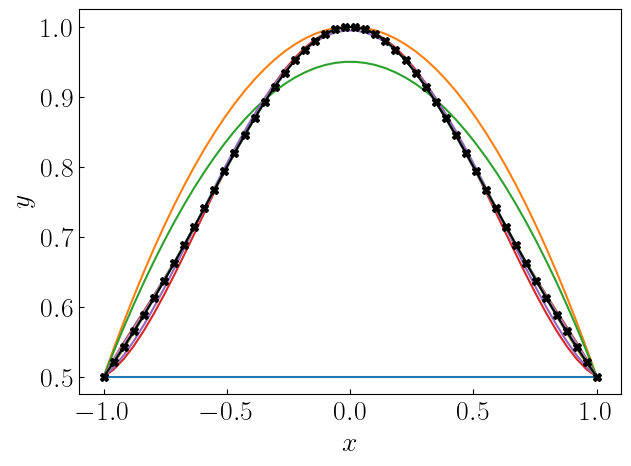
\includegraphics[scale=0.75]{./fig1.png}
    \end{center} 
\end{figure}

Note that the darker marks on the plot highlight the location of $f(x)$.
It can be seen that as more points are added, the interpolating polynomial becomes a better approximation of the function, oscillating about the function with nodes at the data points.

\end{document}
